%%%%%%%%%%%%%%%%%%%%%%%
%%%%%% Lezione 4 %%%%%%
%%%%%%%%%%%%%%%%%%%%%%%

\vspace{1.0cm}
\noindent \lecture{4}{15/10/2021}

\subsection{Atomi a molti elettroni}
\noindent Applichiamo l'equazione di Thomas-Fermi al caso di atomi a molti elettroni. Essi saranno soggetti a:
\begin{equation*}
    V_{\text{ext}}=-\frac{Ze_0^2}{4\pi\varepsilon_0 r}
\end{equation*}
Se andiamo lontani dal nucleo l'equazione si annula 
\begin{equation*}
    \varepsilon_{\text F}(n(x))=\frac{\hbar^2}{2m}(3\pi^2n(x))^{\frac 23}
\end{equation*}
\begin{equation*}
    V_\text{H}(\overline x)=\frac{e_0^2}{4\pi\varepsilon_0}\int \dd[3]{x'}\frac{n(\overline{x}')}{|\overline x - \overline{x}'|}
\end{equation*}
L'equazione di Thomas-Fermi è una equazione che coinvolge integrali in $n(\overline x)$, risulta difficile da risolvere in questa forma. Per risolvere questo problema andiamo a risolvere un'equazione differenziale, non risolviamo questo integrale.\\
Raggruppiamo tutto in un'unico potenziale $V_\text{tot}(\overline x)=V_{\text H}(\overline x)+V_{\text{ext}}(\overline x)$. Osserviamo che è in relazione con l'energia potenziale elettrostatica nel seguente modo:
\begin{equation*}
    V_\text{tot}(\overline x)=-e_0U_\text{el}(\overline x)
\end{equation*}
Esso è legato all'\textbf{equazione di Poisson}:
\begin{equation*}
    \nabla^2U_\text{el}=-\frac{\rho}{\varepsilon_0}=-\frac 1 {\varepsilon_0}(\underbrace{-e_0n(\overline x)}_{\mathclap{\text{Densità \\ elettroni}}}+\underbrace{Ze_0\delta(\overline x)}_{\mathclap{\text{Densità \\ protoni}}})
\end{equation*}
Dalla definizione di potenziale elettrostatico:
\begin{equation*}
    U_\text{el}(\overline x)=-\frac{V_\text{tot}(\overline x)}{e_0}
\end{equation*}
Sostituendo nell'\textbf{equazione di Poisson}:
\begin{equation*}
    \nabla^2V_\text{tot}(\overline x)=-\frac{e_0^2}{\varepsilon_0}n(\overline x)+\frac{Ze_0^2}{\varepsilon_0}\delta(\overline x)
\end{equation*}
Riprendendo l'equazione di Thomas-Fermi, esplicitando l'energia di Fermi possiamo trovare un'espressione per esprimere $n(\overline x)$ in termini del potenziale totale:
\begin{equation*}
    \frac{\hbar^2}{2m}(3\pi^2n(\overline x))^{\frac 23}+V_{\text{tot}}=0
\end{equation*}
\begin{equation*}
    n(\overline x)=\bigg(-V_{\text{tot}}\frac{2m}{\hbar^2}\bigg)^{\frac 32}\frac{1}{3\pi^2}
\end{equation*}
Inserendo questo risultato nell'\textbf{equazione di Poisson}:
\begin{equation*}
    \nabla^2V_{\text{tot}}=-\frac{e_0^2}{\varepsilon_0}\frac{1}{3\pi^2}\bigg(-V_{\text{tot}}\frac{2m}{\hbar^2}\bigg)^{\frac 32}+\frac{Ze_0^2}{\varepsilon_0}\delta(x)
\end{equation*}
A questo punto, prima di risolvere introduciamo le condizioni al contorno:
\begin{equation*}
    \begin{aligned}
    V_{\text{tot}} &\rightarrow - \frac{Ze_0^2}{4\pi\varepsilon_0r}\\
    r &\rightarrow 0
    \end{aligned}
\end{equation*}
\begin{equation*}
    \begin{aligned}
    V_{\text{tot}} &\rightarrow 0\\
    r &\rightarrow +\infty
    \end{aligned}
\end{equation*}
Deve risentire dell'interazione con il nucleo, mentre lontano dal nucleo deve annullarsi, ma deve annullarsi più velocemente di $\frac 1r$
Consideriamo come possibile soluzione:
\begin{equation*}
    \begin{aligned}
        V_{\text{tot}}(r) & =\underbrace{-\frac{Ze_0^2}{4\pi\varepsilon_0r}}_{\mathclap{\text{Contributo del nucleo}}}\chi(r) \\
        & =f(r)\chi(r)
    \end{aligned}
\end{equation*}
\begin{equation*}
    \begin{aligned}
        \chi(r) &\rightarrow  1\\
        r &\rightarrow 0
        \end{aligned}
\end{equation*}
\begin{equation*}
    \begin{aligned}
        \chi(r) &\rightarrow  0\\
        r &\rightarrow +\infty
        \end{aligned}
\end{equation*}
Eseguendo il laplaciano:
\begin{equation*}
    \begin{aligned}
        \nabla^2V_{\text{tot}}(r) & =\nabla\cdot(\nabla f(r)\chi(r)) \\
        & = \nabla \cdot (f\nabla\chi+\nabla f\chi)\\
        & = 2\nabla f \cdot \nabla \chi + f \nabla^2\chi+\chi\nabla^2 f
    \end{aligned}
\end{equation*}
Abbiamo la somma di tre termini, guardando al terzo termine $\chi\nabla^2 f$ ($\chi(r)\rightarrow 1$ per $r\rightarrow 0$) possiamo osservare che corrisponde alla $\delta(x)$ presente nell'\textbf{equazione di Poisson}:
\begin{equation*}
    \chi\nabla^2\bigg(-\frac{Ze_0^2}{4\pi\varepsilon_0r}\bigg)=\frac{Ze_0^2}{\varepsilon_0}\delta(x)
\end{equation*}
Per quanto riguarda gli altri due termini abbiamo:
\begin{equation*}
    2\nabla\bigg(-\frac{Ze_0^2}{4\pi\varepsilon_0r}\bigg)\nabla\chi-\frac{Ze_0^2}{4\pi\varepsilon_0r}\nabla^2\chi=-\frac{e_0^2}{\varepsilon_0}\frac{1}{3\pi^2}\bigg(-\frac{2m}{\hbar^2}V_{\text{tot}}\bigg)^{\frac23}
\end{equation*}
\textbf{Termine} $2\nabla\bigg(-\frac{Ze_0^2}{4\pi\varepsilon_0r}\bigg)\nabla\chi$:
\begin{equation*}
    2\bigg(-\frac{Ze_0^2}{4\pi\varepsilon_0}\bigg)\bigg(-\frac 1{r^2}\bigg)\frac{\overline r}{r}\cdot\frac{\overline r}{r}\chi'=\frac{2Ze_0^2}{4\pi\varepsilon_0r^2}\chi'
\end{equation*}
\textbf{Termine} $-\frac{Ze_0^2}{4\pi\varepsilon_0r}\nabla^2\chi$:
\begin{equation*}
    -\frac{Ze_0^2}{4\pi\varepsilon_0r}\nabla^2\chi=-\frac{Ze_0^2}{4\pi\varepsilon_0r}\bigg(\frac{2\chi'}{r}+\chi''\bigg)
\end{equation*}
Mettendo insieme i due risultati:
\begin{equation*}
    \frac{2Ze_0^2}{4\pi\varepsilon_0r^2}\chi'-\frac{Ze_0^2}{4\pi\varepsilon_0r}\bigg(\frac{2\chi'}{r}+\chi''\bigg)=-\frac{e_0^2}{\varepsilon_0}\frac{1}{3\pi^2}\bigg(-\frac{2m}{\hbar^2}\bigg(-\frac{Ze_0^2}{4\pi\varepsilon_0r}\bigg)\chi\bigg)^{\frac32}
\end{equation*}
\begin{equation*}
    -\frac{Ze_0^2}{4\pi\varepsilon_0r}\chi''=-\frac{e_0^2}{\varepsilon_0}\frac{1}{3\pi^2}\bigg(-\frac{2m}{\hbar^2}\bigg(-\frac{Ze_0^2}{4\pi\varepsilon_0r}\bigg)\chi\bigg)^{\frac32}
\end{equation*}
Semplificando:
\begin{equation*}
    \begin{aligned}
    \chi''& =\frac{4\pi}{Z}\frac{1}{3\pi^2}r\bigg(\frac{2m}{3\hbar^2}\frac{Ze_0^2}{4\pi\varepsilon_0}\bigg)^{\frac32}\frac{1}{r^{\frac32}}\chi^{\frac32}\\
    & = \frac{4\pi}{Z}\frac{1}{3\pi^2}\bigg(\frac{2m}{3\hbar^2}\frac{Ze_0^2}{4\pi\varepsilon_0}\bigg)^{\frac32}\frac{1}{\sqrt r}\chi^{\frac32}
    \end{aligned}
\end{equation*}
Raccogliendo tutte le costanti:
\begin{equation*}
    \chi''=A(Z)\frac{\chi^{\frac32}}{\sqrt r}
\end{equation*}
Supponiamo ora di prendere $r=\alpha x$, dove $\alpha$ è un fattore scalare, avremo:
\begin{equation*}
    \dv[2]{\chi}{r}=\frac{1}{\alpha^2}\dv[2]{\chi}{x}
\end{equation*}
Sostituendo:
\begin{equation*}
    \frac{1}{\alpha^2}\dv[2]{\chi}{x}=A\frac{\chi^{\frac32}}{\sqrt \alpha \sqrt x}\Longrightarrow\dv[2]{\chi}{x}=A\alpha^{\frac 32}\frac{\chi^{\frac32}}{\sqrt x}
\end{equation*}
L'ultima ipotesi che si fa è che il termine $\alpha$ è scelto affinché la quantità $A\alpha^{\frac 32}$ sia costante. Proprio per quest'ultimo risultato abbiamo un'equazione universale per gli atomi:
\begin{equation*}
    \dv[2]{\chi}{x}=\frac{\chi^{\frac 32}}{\sqrt x}
\end{equation*}
Si tratta di una funzione che non possiamo risolvere analiticamente, ma possiamo risolverla numericamente ed è valida per tutti gli atomi.
[GRAFICO ANDAMENTO CHI]
Analizzando i comportamenti asintotici:
\begin{equation*}
    \begin{aligned}
        \chi(x) &\rightarrow  1-1.59x\\
        x &\rightarrow 0
    \end{aligned}
\end{equation*}
\begin{equation*}
    \begin{aligned}
        \chi(x) &\rightarrow  \frac{144}{x^3}\\
        x &\rightarrow +\infty
    \end{aligned}
\end{equation*}
Pertanto dal valore di $\chi(x)$ ricaviamo $V_{\text{tot}}$, da cui poi valutiamo la densità di elettroni $n(\overline x)$ e infine otteniamo l'energia $E\big[n(\overline x)\big]$.
[GRAFICO DENSITÀ RADIALE TRA TF e HF]
Osserviamo che nel metodo di Hartree-Fock la densità radiale va a zero in maniera correttamente esponenziale, mentre nel modello di Thomas-Fermi va come $r^{-6}$.

\chapter{Jellium model: gas omogeneo di elettroni interagenti}
Un modello importante che illustra il ruolo delle interazioni a molti elettroni nei solidi senza dover affrontare la complessità della struttura atomica è quello del gas omogeneo di elettroni interagenti, il \textbf{jellium model}. In questo modello, consideriamo un sistema di elettroni interagenti in un background omogeneo con carica positiva $n_b=n$ in modo che il sistema totale sia neutro. Il \textbf{jellium model} è quindi un metallo idealizzato per il quale possiamo studiare gli effetti delle interazioni degli elettroni sull'energia totale, sulle eccitazioni degli elettroni e su altre proprietà in funzione della densità elettronica.\\
L'energia totale di interazione degli elettroni del jellium è:
\begin{equation*}
    E=T+U_{\text{ee}}+U_{\text{eb}}+U_{\text{bb}}
\end{equation*}
ciascun termine rappresenta l'energia cinetica, l'interazione tra elettroni, l'interazione tra elettroni e background positivo e l'interazione tra background.
$U_{\text{ee}}$ è difficile da conoscere, ma questo contributo può essere scritto come l'\textbf{energia di Hartree} unito a qualcos'altro. Se considerassimo soltanto l'\textbf{energia di Hartree}, la somma di questi termini rappresenta l'energia elettrica totale perché consideriamo tutte le interazioni tra le particelle:
\begin{equation*}
    E_{\text H}+U_{\text{eb}}+U_{\text{bb}}=\frac 12 \int \dd[3]{x'}\dd[3]{x''}\frac{n_{\text{tot}}(\overline{x}')n_{\text{tot}}(\overline{x}'')}{4\pi\varepsilon_0|\overline{x}''-\overline{x}'|}
\end{equation*}
dal momento che il sistema totale è neutro, questa quantità è nulla, proprio perché abbiamo un sistema omogeneo. Consideriamo ora l'\textbf{energia di Hartree-Fock}, scritta come:
\begin{equation*}
    E=\sum_{\mu}\mel{\mu}{\hat T + \underbrace{\hat{V}_{\text{ext}}}_{\mathclap{\text{simile all'interazione eb}}}}{\mu}+\frac 12 \sum_{\mu\nu}\big(J_{\mu\nu}-K_{\mu\nu}\big)+U_{\text{eb}}
\end{equation*}
Se consideriamo questi tre elementi singolarmente, questi termini divergono a $+\infty$. Invece se consideriamo la loro somma, il loro risultato è zero. \\
Allora nel jellium model avremo:
\begin{equation*}
    E=\sum_{\mu}\mel{\mu}{\hat T}{\mu}-\frac 12 \sum_{\mu\nu}K_{\mu\nu}
\end{equation*}
Come al solito, vogliamo minimizzare l'energia scegliendo la funzione d'onda a singola particella adatta:
\begin{equation*}
    \functionalderivative{E_\text{HF}}{u_{\alpha\sigma}^*(\overline x)}=\varepsilon_\alpha u_{\alpha\sigma}(\overline x)
\end{equation*}
\begin{equation*}
    -\frac{\hbar^2}{2m}\nabla^2u_{\alpha\sigma}(\overline x)-\hat V_{\text{F}}u_{\alpha\sigma}(\overline x)=\varepsilon_\alpha u_{\alpha\sigma}(\overline x)
\end{equation*}
In particolare
\begin{equation*}
    \hat V_{\text{F}}u_{\alpha\sigma}(\overline x)=\frac{e_0^2}{4\pi\varepsilon_0}\sum_\nu\int\dd[3]{x'}\frac{u_{\nu\sigma}^*(\overline{x}')u_{\alpha\sigma}(\overline{x}')u_{\nu\sigma}(\overline{x})}{|\overline{x}-\overline{x}'|}
\end{equation*}
$\nu$ rappresenta gli stati occupati, è il set di numeri quantici spaziali, la componente di spin $\sigma$ è la stessa. \\
Dal momento che $[\hat S, \hat H]=0$, la funzione d'onda può essere scritta come: $\psi_{\text{space}}\psi_{\text{spin}}$:
\begin{equation*}
    u_{k\sigma}(\overline x)=\frac{e^{i\overline{k}\cdot\overline{x}}}{\sqrt V}\chi_\sigma \ \ \ \ \ \ \ \ \ \ \overline k=\frac{2\pi}{L}(n_x,n_y,n_z)
\end{equation*}
Inserendo questa soluzione nell'\textbf{equazione di Hartree-Fock}, dimenticandoci della componente di spin perché ininfluente:
\begin{equation*}
    -\frac{\hbar^2}{2m}\nabla^2\frac{e^{i\overline{k}\cdot\overline{x}}}{\sqrt V}-\sum_{\mathclap{\overline{k}'<\overline{k}_\text{F}}}\dd[3]{x'}e^{-i\overline{k}'\cdot\overline{x}'}e^{i\overline{k}\cdot\overline{x}'}e^{i\overline{k}'\cdot\overline{x}}\frac{e_0^2}{4\pi\varepsilon_0|\overline{x}-\overline{x}'|}\frac{1}{V^{\frac 32}}=\varepsilon_{\overline k}\frac{e^{i\overline{k}\cdot\overline{x}}}{\sqrt V}
\end{equation*}
Supponiamo ora di introdurre il seguente termine sotto l'integrale:
\begin{equation*}
    e^{i\overline{k}\cdot\overline{x}}e^{-i\overline{k}\cdot\overline{x}}=1
\end{equation*}
Osserviamo che non cambia l'integrale:
\begin{equation*}
    \int \dd[3]{x'}e^{-i\overline{k}'\cdot(\overline{x}'-\overline{x})}e^{i\overline{k}\cdot(\overline{x}'-\overline{x})}e^{i\overline{k}\cdot\overline{x}} = -\sum_{|\overline{k}'|<k_F}\int \dd[3]{x'}\frac{e^{i(\overline{k}-\overline{k}')\cdot(\overline{x}'-\overline{x})}}{V|\overline{x}-\overline{x}'|}\frac{e_0^2}{4\pi\varepsilon_0}\frac{e^{i\overline{k}\cdot\overline{x}}}{\sqrt V}
\end{equation*}
Facendo un cambio di variabile $\overline{y}=\overline{x}-\overline{x}'$
\begin{equation*}
    -\sum_{|\overline{k}'|<k_F}\int\dd[3]{y}\frac{e^{i(\overline k -\overline k')\cdot\overline y}}{V|\overline y|}\frac{e_0^2}{4\pi\varepsilon_0}\frac{e^{i\overline k \cdot \overline x}}{\sqrt V}
\end{equation*}
Questa non è nient'altro che la trasformata di Fourier per $\frac{1}{|\overline y|}$:
\begin{equation*}
    \int \dd[3]{q}e^{i\overline q \cdot \overline y}\frac{1}{|\overline y|}=\frac{4\pi}{q^2}
\end{equation*}
Inserendo questo risultato:
\begin{equation*}
    \underbrace{-\frac{e_0^2}{4\pi\varepsilon_0}\sum_{|\overline{k}'|<k_F}\frac{4\pi}{|\overline k - \overline k '|^2}\frac{1}{V}}_{E_\text{X}(\overline k)}\underbrace{\frac{e^{i\overline k \cdot \overline x}}{\sqrt V}}_{u_{\overline k}(\overline x)}=-\hat V_{\text F}u_{\overline k}(\overline x)
\end{equation*}
\begin{equation*}
    \frac{\hbar^2k^2}{2m}\frac{e^{i\overline k \cdot \overline x}}{\sqrt V}+E_{\text X}(\overline k)\frac{e^{i\overline k \cdot \overline x}}{\sqrt V}=\varepsilon_{\overline k}\frac{e^{i\overline k \cdot \overline x}}{\sqrt V}
\end{equation*}
Quindi l'energia sarà:
\begin{equation*}
    \varepsilon(k)=\frac{\hbar^2k^2}{2m}+E_{\text X}(k)
\end{equation*}
Sotto l'ipotesi di un gran numero di particelle possiamo passare dalla sommatoria $\sum$ all'integrale $\int$:
\begin{equation*}
    \sum_{\overline k'} \rightarrow \int \frac{\dd[3]{k'}V}{(2\pi)^3}
\end{equation*}
\begin{equation*}
    \begin{aligned}
        E_{\text X}(k) & =-\frac{e_0^2}{\varepsilon}\sum_{|\overline k'|<k_F}\frac{1}{|\overline k - \overline k'|^2}\frac{1}{V} \\
        & = -\frac{e_0^2}{\varepsilon}\int_{\mathclap{|\overline k'|<k_F}}\dd[3]{k'}\frac{1}{|\overline k - \overline k'|^2} \\
        & = - \frac{e_0^2}{\varepsilon_0}\int_0^{2\pi}\dd{\phi}\int_0^\pi\dd{\theta}\sin\theta\int_0^{k_{\text F}}\dd{k'}{k'}^2\frac{1}{{k'}^2+k^2-2kk'\sin\theta}\\
        & = \dots\\
        & = -\frac{e_0^2}{\varepsilon_0}\frac{1}{(2\pi)^2}2{k}_{\text{F}}F\bigg(\frac{k}{k_{\text F}}\bigg)\\
    \end{aligned}
\end{equation*}
dove
\begin{equation*}
    F(x)=\frac 12 + \frac{(1-x^2)}{4x}\ln\Bigg|\frac{1+x}{1-x}\Bigg|    
\end{equation*}
\begin{figure}[!ht]
    \centering
    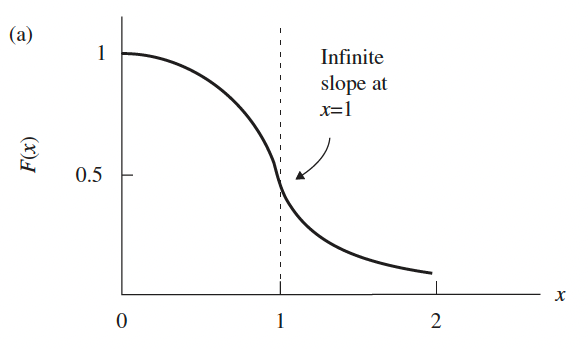
\includegraphics[scale=0.6]{images/F(x)jellium.png}
    \caption{Andamento di $F(x)$ con singolarità logaritmica in $x=1$}
    \label{fig:fxjellium}
\end{figure}
\newpage
\begin{figure}[!ht]
    \centering
    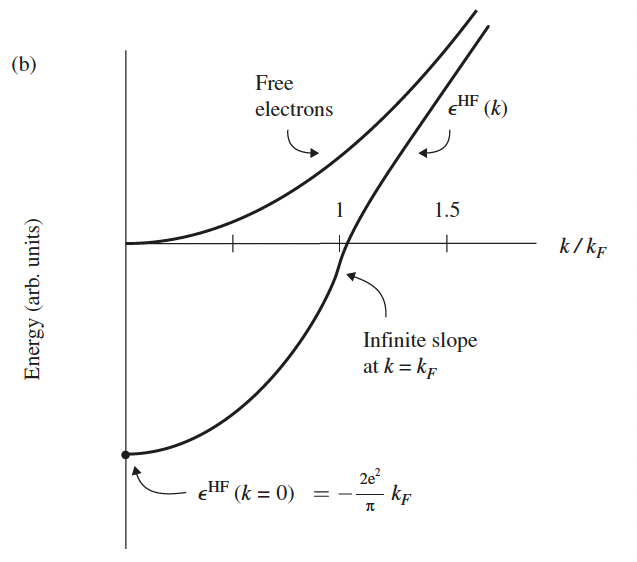
\includegraphics[scale=0.6]{images/energyjellium.png}
    \caption{Energia di Hartree-Fock per un gas di elettroni interagenti confrontata con l'energia di un gas di elettroni liberi}
    \label{fig:energyjellium}
\end{figure}
\begin{equation*}
    \varepsilon_{\text{HF}}(\overline k)=\frac{\hbar^2k^2}{2m}+E_{\text X}(k)
\end{equation*}
Osserviamo che la velocità della funzione d'onda è definita come:
\begin{equation*}
    \overline v = \frac{1}{\hbar}\partialderivative{\varepsilon(\overline k)}{\overline k}
\end{equation*}
Per via del fatto che nella definizione di $F(x)$ c'è un punto di flesso verticale, la velocità diverge a $k_{\text F}$ nel metodo di \textbf{Hartree-Fock}, il che non è buono. La velocità sulla sfera di Fermi controlla i sistemi elettrici e non possiamo avere $v \rightarrow +\infty$. Quindi il \textbf{metodo di Hartree-Fock} non si comporta molto bene in questo modello. Ciò che manca è l'\textbf{energia di correlazione}.
